% !TEX program = xelatex
\documentclass{article}

\title{Notite examen - Algoritmi Fundamentali}
\date{}
\author{Dinu Florin-Silviu \\ grupa 231}

\newcommand{\prim}{^\ensuremath{\prime}}
\newcommand{\secund}{^{\ensuremath{\prime\prime}}}

% \makeatletter
% \renewcommand{\@seccntformat}[1]{}
% \makeatother

\newenvironment{textColor}[1]{%
    \leavevmode\color{#1}\ignorespaces%
}{%
}%


\usepackage{tikz}
\usepackage{forest}
\usepackage{hyperref}
\usepackage{amsthm}
\usepackage{amssymb}
\usepackage[english]{babel}
\usepackage[a4paper, margin=3cm]{geometry}
\usepackage{enumitem}
\usepackage{listings}
\usepackage{fontspec}
\usepackage{xcolor}
\usepackage{textcomp}
\usepackage{graphicx}
\usepackage{tabularx}

\graphicspath{ {./img/} }

\newfontfamily{\ttconsolas}{Consolas}
\lstset{
%  tabsize=4,
extendedchars=true,
        basicstyle=\ttconsolas,
        % %upquote=false,
        % aboveskip=\baselineskip,
        columns=fixed,
        showstringspaces=false,
        extendedchars=true,
        breaklines=true,
        % prebreak = \raisebox{0ex}[0ex][0ex]{\ensuremath{\hookleftarrow}},
        showtabs=false,
        showspaces=false,
        identifierstyle=\ttfamily,
        % keywordstyle=\color[rgb]{0,0,1},
        % commentstyle=\color[rgb]{0.133,0.545,0.133},
        % stringstyle=\color[rgb]{0.627,0.126,0.941},
        % language=SQL
        frame=lines,
        literate=%
    {€}{\euro}1%
    {§}{\S}1%
    {°}{\textdegree{}}1%
    {ä}{{\"a}}1%
    {ö}{{\"o}}1%
    {ü}{{\"u}}1%
    {ß}{{\ss}}1%
    {Ä}{{\"A}}1%
    {Ö}{{\"O}}1%
    {Ü}{{\"U}}1%
    {µ}{\textmu}1%
    {¹}{{\textsuperscript{1}}}1%
    {²}{{\textsuperscript{2}}}1%
    {³}{{\textsuperscript{3}}}1%
    {¼}{\textonequarter}1%
    {½}{\textonehalf}1%
    {¢}{\textcent}1%
}


\tikzstyle{red state}=[
        draw = red,
        thick,
        fill = white,
        minimum size = 4mm,
        circle
    ]

\tikzstyle{blue state}=[
    draw = blue,
    thick,
    fill = white,
    minimum size = 4mm,
    circle
]

\tikzstyle{green state}=[
    draw = green,
    thick,
    fill = white,
    minimum size = 4mm,
    circle
]

\newtheorem*{theorem}{Teorema}
\renewcommand\qedsymbol{QED}

\begin{document}
\pagenumbering{gobble}
\maketitle
\tableofcontents

\newpage
\pagenumbering{arabic}

\section{Notiuni fundamentale}
\subsection*{Grafuri izomorfe} Daca 2 grafuri:
\begin{itemize}
    \item Au acelasi numar de noduri
    \item Au acelasi numar de muchii
    \item Nodurile formeaza o secventa cu acelasi grad
    \item Daca un graf are un ciclu de lungime k, si celalalt graf are la fel
\end{itemize}

\subsection*{Grafuri bipartite} Daca un graf:
\begin{itemize}
    \item Neorientat
    \item Putem imparti nodurile in 2 multimi $V=V_1 \cup V_2$ cu $V_1 \cap V_2 = \varnothing$
    \item Fiecare muchie are o extremitate intr-o parte si cealalta in cealalta parte, adica $|e \cap V_1| = |e \cap V_2| = 1$
\end{itemize}

\subsection*{Construire graf cu secventa gradelor (Havel-Hakimi)} Ordonam descrescator gradele si incepem sa trasam muchii catre urmatoarele, scazand din gradele lor pana cand ajungem sa avem doar 0. Daca avem $d_i<0$ sau $d_i>n-1$ sau $(\sum_{i=0}^{n} d_i) \% 2 = 1$ atunci nu are solutie.

\section{Parcurgeri}
\subsection*{BFS} Se iau toti vecinii nevizitati, se pun in coada, se continua cu urmatorul din coada. Complexitate $O(V+E)$. Se foloseste pentru iesirea din labirint cu drum minim si calcul nivel.
\begin{lstlisting}
void bfs(vector<vector<int>> &lista, vector<int> &pbfs, queue<int> &q) {
    int s = q.front();
    q.pop();

    int nivel = pbfs[s] + 1;

    for (auto x: lista[s]) {
        if (pbfs[x] == -1) {
            pbfs[x] = nivel;
            q.push(x);
        }
    }

    if (q.empty()) return;

    bfs(lista, pbfs, q);
}
    \end{lstlisting}

\begin{itemize}
    \item Muchiile de arbore sunt muchii din pădurea de adâncime $G_\pi$. Muchia (u, v) este o muchie de arbore dacă v a fost descoperit explorând muchia (u, v).
    \item Muchiile înapoi sunt acele muchii (u, v) care unesc un vârf u cu un strămoş v într-un arbore de adâncime. Buclele (muchii de la un vârf la el însuşi) care pot apărea într-un graf orientat sunt considerate muchii înapoi.
    \item Muchiile înainte sunt acele muchii (u, v) ce nu sunt muchii de arbore şi conectează un vârf u cu un descendent v într-un arbore de adâncime.
    \item Muchiile transversale sunt toate celelalte muchii. Ele pot uni vârfuri din acelaşi arbore de adâncime, cu condiţia ca unul să nu fie strămoşul celuilalt, sau pot uni vârfuri din arbori, de adâncime, diferiţi.
\end{itemize}

\subsection*{DFS} Complexitate $O(V+E)$.
\begin{lstlisting}
void Graph::DFS(int v)
{
    // Mark the current node as visited and
    // print it
    visited[v] = true;
    cout << v << " ";
 
    // Recur for all the vertices adjacent
    // to this vertex
    list<int>::iterator i;
    for (i = adj[v].begin(); i != adj[v].end(); ++i)
        if (!visited[*i])
            DFS(*i);
}
    \end{lstlisting}

\section{Sortare topologica}
Se face pe DAG (directed acyclic graph)
\subsection*{Cu BFS} Incepe de la toate nodurile care au $indegree == 0$ (DAG garanteaza cel putin 1 astfel de nod). Dupa ce scoatem nodul din coada, il punem in vector.
\begin{lstlisting}
vector<int> topo(int N, vector<int> adj[]) {
    queue<int> q; 
    vector<int> indegree(N, 0); 
    for(int i = 0;i<N;i++) {
        for(auto it: adj[i]) {
            indegree[it]++; 
        }
    }
    
    for(int i = 0;i<N;i++) {
        if(indegree[i] == 0) {
            q.push(i); 
        }
    }
    vector<int> topo;
    while(!q.empty()) {
        int node = q.front(); 
        q.pop(); 
        topo.push_back(node);
        for(auto it : adj[node]) {
            indegree[it]--;
            if(indegree[it] == 0) {
                q.push(it); 
            }
        }
    }
    return topo;
}
    \end{lstlisting}
\subsection*{Cu DFS} Diferentea fata de DFS e ca pun la sfarsit nodul pe stack. Diferentele fata de anterior sunt ca iau tot ce nu e vizitat si ca e mai eficient dpdv al memoriei, cat timp lantul cel mai lung nu da stackoverflow. Complexitate $O(V+E)$

\begin{lstlisting}
void Graph::topologicalSortUtil(int v, bool visited[],
                                stack<int>& Stack)
{
    // Mark the current node as visited.
    visited[v] = true;
 
    // Recur for all the vertices
    // adjacent to this vertex
    list<int>::iterator i;
    for (i = adj[v].begin(); i != adj[v].end(); ++i)
        if (!visited[*i])
            topologicalSortUtil(*i, visited, Stack);
 
    // Push current vertex to stack
    // which stores result
    Stack.push(v);
}
    \end{lstlisting}

\section{Muchii critice} Acele muchii care nu fac parte dintr-un ciclu. Facem un DFS si tinem 2 valori: low si disc. Pentru fiecare nod, mai intai punem disc ca fiind $disc_anterior + 1$, trecem la copil, pentru el memoram parintele, apoi facem DFS, apoi actualizam low ca fiind $min(low[copil], low[parinte])$. Daca este critica, atunci $low[copil]>disc[parinte]$.
\begin{lstlisting}
void Graph::bridgeUtil(int u, bool visited[], int disc[],
                                  int low[], int parent[])
{
    // A static variable is used for simplicity, we can
    // avoid use of static variable by passing a pointer.
    static int time = 0;
 
    // Mark the current node as visited
    visited[u] = true;
 
    // Initialize discovery time and low value
    disc[u] = low[u] = ++time;
 
    // Go through all vertices adjacent to this
    list<int>::iterator i;
    for (i = adj[u].begin(); i != adj[u].end(); ++i)
    {
        int v = *i;  // v is current adjacent of u
 
        // If v is not visited yet, then recur for it
        if (!visited[v])
        {
            parent[v] = u;
            bridgeUtil(v, visited, disc, low, parent);
 
            // Check if the subtree rooted with v has a
            // connection to one of the ancestors of u
            low[u]  = min(low[u], low[v]);
 
            // If the lowest vertex reachable from subtree
            // under v is  below u in DFS tree, then u-v
            // is a bridge
            if (low[v] > disc[u])
              cout << u <<" " << v << endl;
        }
 
        // Update low value of u for parent function calls.
        else if (v != parent[u])
            low[u]  = min(low[u], disc[v]);
    }
}
    \end{lstlisting}

\section{Puncte critice} V este punct critic, daca exista 2 noduri x si y, cu $x,y \neq v$, pentru care v apartine oricarui $x,y-lant$

\begin{lstlisting}
void APUtil(vector<int> adj[], int u, bool visited[],
            int disc[], int low[], int& time, int parent,
            bool isAP[])
{
    // Count of children in DFS Tree
    int children = 0;
 
    // Mark the current node as visited
    visited[u] = true;
 
    // Initialize discovery time and low value
    disc[u] = low[u] = ++time;
 
    // Go through all vertices adjacent to this
    for (auto v : adj[u]) {
        // If v is not visited yet, then make it a child of u
        // in DFS tree and recur for it
        if (!visited[v]) {
            children++;
            APUtil(adj, v, visited, disc, low, time, u, isAP);
 
            // Check if the subtree rooted with v has
            // a connection to one of the ancestors of u
            low[u] = min(low[u], low[v]);
 
            // If u is not root and low value of one of
            // its child is more than discovery value of u.
            if (parent != -1 && low[v] >= disc[u])
                isAP[u] = true;
        }
 
        // Update low value of u for parent function calls.
        else if (v != parent)
            low[u] = min(low[u], disc[v]);
    }
 
    // If u is root of DFS tree and has two or more children.
    if (parent == -1 && children > 1)
        isAP[u] = true;
}
    \end{lstlisting}

\section{Conexitate in graf orientat} Exista 2 tipuri de conexitati intr-un graf orientat:
\begin{itemize}
    \item Slab conex: Drum de intre $\forall$ 2 noduri daca consideram graful neorientat
    \item Tare conex: Drum intre $\forall$ 2 noduri
\end{itemize}

\subsection*{Kosaraju} Fac un DFS in care adaug pe stack nodurile. Transpun graful. Popuiesc stackul, fac DFS pe acel nod in care marchez elementele ca vizitate, apoi popuiesc urmatorul element si fac DFS daca e nevizitat. Complexitate $O(V+E)$.

\begin{lstlisting}
#include <bits/stdc++.h>

#define MAX_N 20001
#define ll long long int
using namespace std;
int n, m;

struct Node {
  vector < int > adj;
  vector < int > rev_adj;
};

Node g[MAX_N];

stack < int > S;
bool visited[MAX_N];

int component[MAX_N];
vector < int > components[MAX_N];
int numComponents;

void dfs_1(int x) {
  visited[x] = true;
  for (int i = 0; i < g[x].adj.size(); i++) {
    if (!visited[g[x].adj[i]]) dfs_1(g[x].adj[i]);
  }
  S.push(x);
}

void dfs_2(int x) {
  printf("%d ", x);
  component[x] = numComponents;
  components[numComponents].push_back(x);
  visited[x] = true;
  for (int i = 0; i < g[x].rev_adj.size(); i++) {
    if (!visited[g[x].rev_adj[i]]) dfs_2(g[x].rev_adj[i]);
  }
}

void Kosaraju() {
  for (int i = 0; i < n; i++)
    if (!visited[i]) dfs_1(i);

  for (int i = 0; i < n; i++)
    visited[i] = false;

  while (!S.empty()) {
    int v = S.top();
    S.pop();
    if (!visited[v]) {
      printf("Component %d: ", numComponents);
      dfs_2(v);
      numComponents++;
      printf("\n");
    }
  }
}

int main() {

  cin >> n >> m;
  int a, b;
  while (m--) {
    cin >> a >> b;
    g[a].adj.push_back(b);
    g[b].rev_adj.push_back(a);
  }

  Kosaraju();
  printf("Total number of components: %d\n", numComponents);

  return 0;
}

    \end{lstlisting}

\subsection*{Lema} Dacă două vârfuri se află în aceeaşi componentă tare conexă, atunci
nici un drum între ele nu părăseşte, vreodată, componentă tare conexă.
\\
\textbf{Demonstrație:} Fie u și v două noduri din componenta tare conexă.
Presupunem ca exista w în afara componentei și există drum u - > v prin w.
Atunci avem drum de la u la w dar avem și drumul w->v->u deci și drum de la
w la u deci w este în componenta tare conexă.

\section{APM - arbori partiali de cost minim}
\subsection*{Kruskal} $O(E*log E+ E*log V)$ Algoritmul are 3 pasi:
\begin{itemize}
    \item Sorteaza toate muchiile in oridinea crescatoare a greutatii
    \item Alege muchia cea mai mica, daca formeaza un ciclu, treci la urmatoarea, daca nu, adaug-o.
    \item Repeta pasul anterior pana ai $V - 1$ muchii.
\end{itemize}

\paragraph*{Exemplu} Fie graful

\begin{center}
    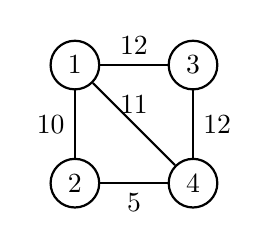
\begin{tikzpicture}[node distance={15mm}, thick, main/.style = {draw, circle}]
        \node[main] (1) {1};
        \node[main] (2) [below of = 1] {2};
        \node[main] (3) [right of = 1] {3};
        \node[main] (4) [below of = 3]{4};

        \draw[-] (1) -- (2) node [midway,left] {10};
        \draw[-] (2) -- (4) node [midway, below] {5};
        \draw[-] (3) -- (4) node [midway, right] {12};
        \draw[-] (1) -- (4) node [midway, right, above] {11};
        \draw[-] (1) -- (3) node [midway, above] {12};

    \end{tikzpicture}
\end{center}

\subparagraph*{Pasul 1.} Sortam ASC muchiile: $\{(2,4,5), (1,2,10), (1,4,11), (1,3,12), (3,4,12)\}$. Am folosit notatia $(nod1, nod2, greutate)$.
\subparagraph*{Pasii 2 \& 3.}
\subparagraph*{1.} Incepem recursia alegand cea mai mica muchie $(2,4,5)$.

\begin{center}
    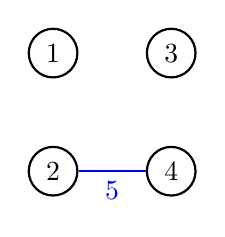
\begin{tikzpicture}[node distance={15mm}, thick, main/.style = {draw, circle}]
        \node[main] (1) {1};
        \node[main] (2) [below of = 1] {2};
        \node[main] (3) [right of = 1] {3};
        \node[main] (4) [below of = 3]{4};

        \draw[blue] (2) -- (4) node [midway, below] {5};

    \end{tikzpicture}
\end{center}

\subparagraph*{2.} Continuam cu $(1,2,10)$.

\begin{center}
    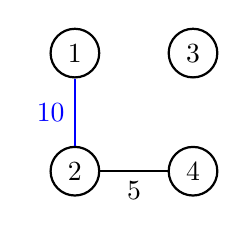
\begin{tikzpicture}[node distance={15mm}, thick, main/.style = {draw, circle}]
        \node[main] (1) {1};
        \node[main] (2) [below of = 1] {2};
        \node[main] (3) [right of = 1] {3};
        \node[main] (4) [below of = 3]{4};

        \draw[-] (2) -- (4) node [midway, below] {5};
        \draw[blue] (1) -- (2) node [midway,left] {10};

    \end{tikzpicture}
\end{center}

\subparagraph*{3.} Continuam cu $(1,4,11)$.

\begin{center}
    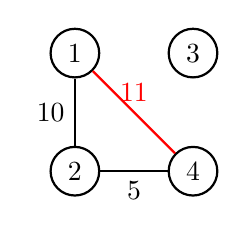
\begin{tikzpicture}[node distance={15mm}, thick, main/.style = {draw, circle}]
        \node[main] (1) {1};
        \node[main] (2) [below of = 1] {2};
        \node[main] (3) [right of = 1] {3};
        \node[main] (4) [below of = 3]{4};

        \draw[-] (2) -- (4) node [midway, below] {5};
        \draw[-] (1) -- (2) node [midway,left] {10};
        \draw[red] (1) -- (4) node [midway, right, above] {11};

    \end{tikzpicture}
\end{center}

\begin{center}
    \textbf{Observam ca face ciclu, deci o ignoram}
\end{center}

\begin{center}
    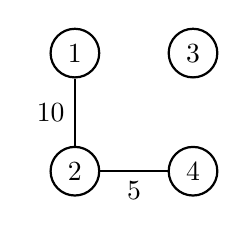
\begin{tikzpicture}[node distance={15mm}, thick, main/.style = {draw, circle}]
        \node[main] (1) {1};
        \node[main] (2) [below of = 1] {2};
        \node[main] (3) [right of = 1] {3};
        \node[main] (4) [below of = 3]{4};

        \draw[-] (2) -- (4) node [midway, below] {5};
        \draw[-] (1) -- (2) node [midway,left] {10};

    \end{tikzpicture}
\end{center}

\subparagraph*{4.} Continuam cu $(1,3,12)$.

\begin{center}
    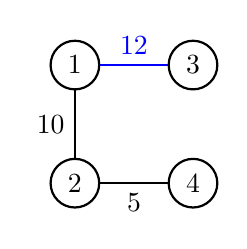
\begin{tikzpicture}[node distance={15mm}, thick, main/.style = {draw, circle}]
        \node[main] (1) {1};
        \node[main] (2) [below of = 1] {2};
        \node[main] (3) [right of = 1] {3};
        \node[main] (4) [below of = 3]{4};

        \draw[-] (2) -- (4) node [midway, below] {5};
        \draw[-] (1) -- (2) node [midway,left] {10};
        \draw[blue] (1) -- (3) node [midway, above] {12};

    \end{tikzpicture}
\end{center}

\begin{center}
    \textbf{Observam ca avem $V-1$ muchii, deci ramanem cu acest graf}
\end{center}

\subparagraph*{K-clustering (aplicatie)} Imparte in k clustere (are $n-k$ pasi)
\begin{center}
    \includegraphics[scale=0.3]{1_kclustering.png}
\end{center}

\subsection*{Prim} Complexitate $O(V^2)$ sau $O(V*logV + E*logV)$ daca folosim minheap. Algoritmul are 6 pasi:
\begin{itemize}
    \item Alegem un nod $n$ aleatoriu si il scoatem din lista nodurilor de ales
    \item Adaugam in structura de date toti vecinii sai impreuna cu greutatea muchiilor
    \item Actualizam eticheta pentru fiecare varf cu distanta minima fata de cele incluse in graf
    \item Adaugam nodul cu distanta minima cea mai mica, il scaotem din lista nodurilor de ales si ii facem parintele nodul de care se leaga
    \item Adaugam in structura de date toti vecinii sai impreuna cu greutatea muchiilor
    \item Repetam al 4-lea pas.
\end{itemize}

\begin{center}
    \includegraphics*[scale=0.3]{2_prim.png}
\end{center}
\begin{center}
    \textbf{$\uparrow$ Prim prin vector vizitat $\uparrow$}
\end{center}


\paragraph*{Exemplu} Fie graful

\begin{center}
    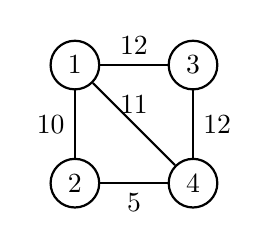
\begin{tikzpicture}[node distance={15mm}, thick, main/.style = {draw, circle}]
        \node[main] (1) {1};
        \node[main] (2) [below of = 1] {2};
        \node[main] (3) [right of = 1] {3};
        \node[main] (4) [below of = 3]{4};

        \draw[-] (1) -- (2) node [midway,left] {10};
        \draw[-] (2) -- (4) node [midway, below] {5};
        \draw[-] (3) -- (4) node [midway, right] {12};
        \draw[-] (1) -- (4) node [midway, right, above] {11};
        \draw[-] (1) -- (3) node [midway, above] {12};

    \end{tikzpicture}
\end{center}

\subparagraph*{Pasul 1.} Plecam de la nodul 1 si facem urmatoarea structura

\begin{center}
    $[(d/tata)] = \{(0,0),(\infty,0),(\infty,0),(\infty,0)\}$
\end{center}

\subparagraph*{Pasul 2.}
\begin{center}
    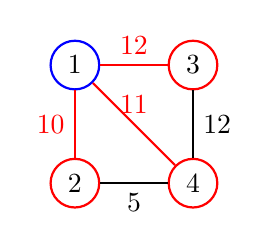
\begin{tikzpicture}[node distance={15mm}, thick, main/.style = {draw, circle}]
        \node[blue state] (1) {1};
        \node[red state] (2) [below of = 1] {2};
        \node[red state] (3) [right of = 1] {3};
        \node[red state] (4) [below of = 3]{4};

        \draw[red] (1) -- (2) node [midway,left] {10};
        \draw[-] (2) -- (4) node [midway, below] {5};
        \draw[-] (3) -- (4) node [midway, right] {12};
        \draw[red] (1) -- (4) node [midway, right, above] {11};
        \draw[red] (1) -- (3) node [midway, above] {12};

    \end{tikzpicture}
\end{center}

\subparagraph*{Pasul 3.}
\begin{center}
    $[(d/tata)] = \{(0,0),(10,0),(12,0),(11,0)\}$
\end{center}

\subparagraph*{Pasul 4.}
\begin{center}
    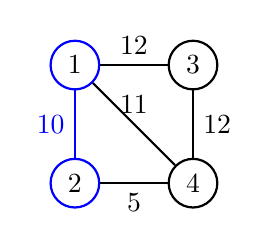
\begin{tikzpicture}[node distance={15mm}, thick, main/.style = {draw, circle}]
        \node[blue state] (1) {1};
        \node[blue state] (2) [below of = 1] {2};
        \node[main] (3) [right of = 1] {3};
        \node[main] (4) [below of = 3]{4};

        \draw[blue] (1) -- (2) node [midway,left] {10};
        \draw[-] (2) -- (4) node [midway, below] {5};
        \draw[-] (3) -- (4) node [midway, right] {12};
        \draw[-] (1) -- (4) node [midway, right, above] {11};
        \draw[-] (1) -- (3) node [midway, above] {12};

    \end{tikzpicture}
\end{center}

\subparagraph*{Pasul 5.}

\begin{center}
    $[(d/tata)] = \{(0,0),(10,1),(12,0),(5,0)\}$
\end{center}

\subparagraph*{Pasul 6. Repetam}

\begin{center}
    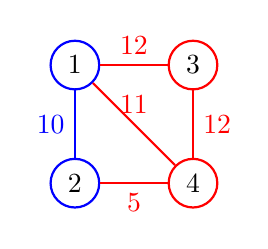
\begin{tikzpicture}[node distance={15mm}, thick, main/.style = {draw, circle}]
        \node[blue state] (1) {1};
        \node[blue state] (2) [below of = 1] {2};
        \node[red state] (3) [right of = 1] {3};
        \node[red state] (4) [below of = 3]{4};

        \draw[blue] (1) -- (2) node [midway,left] {10};
        \draw[red] (2) -- (4) node [midway, below] {5};
        \draw[red] (3) -- (4) node [midway, right] {12};
        \draw[red] (1) -- (4) node [midway, right, above] {11};
        \draw[red] (1) -- (3) node [midway, above] {12};

    \end{tikzpicture}
\end{center}

\begin{center}
    $[(d/tata)] = \{(0,0),(10,1),(12,0),(5,0)\}$
\end{center}

\begin{center}
    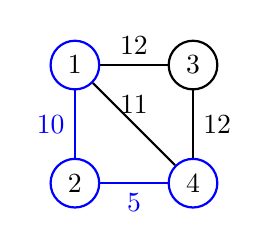
\begin{tikzpicture}[node distance={15mm}, thick, main/.style = {draw, circle}]
        \node[blue state] (1) {1};
        \node[blue state] (2) [below of = 1] {2};
        \node[main] (3) [right of = 1] {3};
        \node[blue state] (4) [below of = 3]{4};

        \draw[blue] (1) -- (2) node [midway,left] {10};
        \draw[blue] (2) -- (4) node [midway, below] {5};
        \draw[-] (3) -- (4) node [midway, right] {12};
        \draw[-] (1) -- (4) node [midway, right, above] {11};
        \draw[-] (1) -- (3) node [midway, above] {12};

    \end{tikzpicture}
\end{center}

\begin{center}
    $[(d/tata)] = \{(0,0),(10,1),(12,0),(5,2)\}$
\end{center}

\begin{center}
    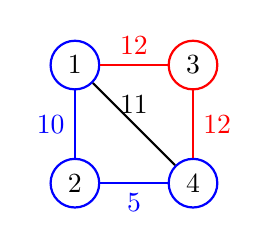
\begin{tikzpicture}[node distance={15mm}, thick, main/.style = {draw, circle}]
        \node[blue state] (1) {1};
        \node[blue state] (2) [below of = 1] {2};
        \node[red state] (3) [right of = 1] {3};
        \node[blue state] (4) [below of = 3]{4};

        \draw[blue] (1) -- (2) node [midway,left] {10};
        \draw[blue] (2) -- (4) node [midway, below] {5};
        \draw[red] (3) -- (4) node [midway, right] {12};
        \draw[-] (1) -- (4) node [midway, right, above] {11};
        \draw[red] (1) -- (3) node [midway, above] {12};

    \end{tikzpicture}
\end{center}

\begin{center}
    $[(d/tata)] = \{(0,0),(10,1),(12,0),(5,2)\}$
\end{center}

\begin{center}
    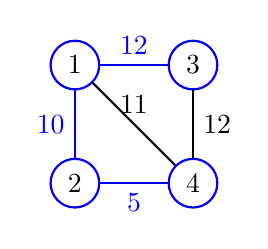
\begin{tikzpicture}[node distance={15mm}, thick, main/.style = {draw, circle}]
        \node[blue state] (1) {1};
        \node[blue state] (2) [below of = 1] {2};
        \node[blue state] (3) [right of = 1] {3};
        \node[blue state] (4) [below of = 3]{4};

        \draw[blue] (1) -- (2) node [midway,left] {10};
        \draw[blue] (2) -- (4) node [midway, below] {5};
        \draw[-] (3) -- (4) node [midway, right] {12};
        \draw[-] (1) -- (4) node [midway, right, above] {11};
        \draw[blue] (1) -- (3) node [midway, above] {12};

    \end{tikzpicture}
\end{center}

\begin{center}
    $[(d/tata)] = \{(0,0),(10,1),(12,1),(5,2)\}$
\end{center}

\begin{center}
    \textbf{APM final}
\end{center}

\begin{center}
    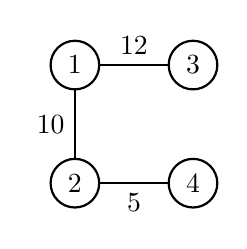
\begin{tikzpicture}[node distance={15mm}, thick, main/.style = {draw, circle}]
        \node[main] (1) {1};
        \node[main] (2) [below of = 1] {2};
        \node[main] (3) [right of = 1] {3};
        \node[main] (4) [below of = 3]{4};

        \draw[-] (1) -- (2) node [midway,left] {10};
        \draw[-] (2) -- (4) node [midway, below] {5};
        \draw[-] (1) -- (3) node [midway, above] {12};

    \end{tikzpicture}
\end{center}

\begin{center}
    \includegraphics*[scale=0.3]{3_prim_minheap.png}
\end{center}
\begin{center}
    \textbf{$\uparrow$ Prim prin minheap $\uparrow$}
\end{center}

\section{Drumuri minime de sursa unica \textit{s}}
\subsection*{Dijkstra}
Se poate folosi doar pentru drumuri de cost pozitiv
\paragraph*{Complexitate}
\begin{itemize}
    \item Cu heap $O(E*logV)$
          \begin{itemize}
              \item Initializare Q: $O(n)$
              \item n * extragere varf minim: $O(n*log\ n)$
              \item Actualizare etichete vecini: $O(n*log\ n)$
          \end{itemize}
    \item Cu vector $O(V^2)$
          \begin{itemize}
              \item Initializare Q: $O(n)$
              \item n * extragere varf minim: $O(n^2)$
              \item Actualizare etichete vecini: $O(m^2)$
          \end{itemize}
\end{itemize}
\begin{center}
    \includegraphics[scale=0.3]{4_dijkstra.png}
\end{center}
\begin{center}
    \textbf{$\uparrow$ Dijskstra cu min heap $\uparrow$}
\end{center}

\begin{center}
    \includegraphics[scale=0.3]{5_dijkstra_vector.png}
\end{center}
\begin{center}
    \textbf{$\uparrow$ Dijskstra cu vector $\uparrow$}
\end{center}

\paragraph*{Exemplu} Fie graful in care incepem de la 1.

\begin{center}
    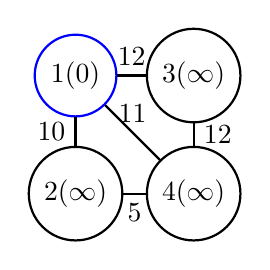
\begin{tikzpicture}[node distance={15mm}, thick, main/.style = {draw, circle}]
        \node[blue state] (1) {1(0)};
        \node[main] (2) [below of = 1] {2($\infty$)};
        \node[main] (3) [right of = 1] {3($\infty$)};
        \node[main] (4) [below of = 3]{4($\infty$)};

        \draw[-] (1) -- (2) node [midway,left] {10};
        \draw[-] (2) -- (4) node [midway, below] {5};
        \draw[-] (3) -- (4) node [midway, right] {12};
        \draw[-] (1) -- (4) node [midway, right, above] {11};
        \draw[-] (1) -- (3) node [midway, above] {12};

    \end{tikzpicture}
\end{center}

\subparagraph*{Consideram vecinii lui 1}
\begin{center}
    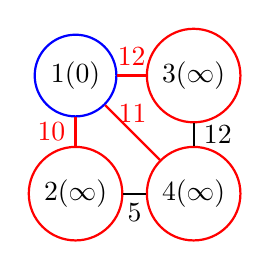
\begin{tikzpicture}[node distance={15mm}, thick, main/.style = {draw, circle}]
        \node[blue state] (1) {1(0)};
        \node[red state] (2) [below of = 1] {2($\infty$)};
        \node[red state] (3) [right of = 1] {3($\infty$)};
        \node[red state] (4) [below of = 3]{4($\infty$)};

        \draw[red] (1) -- (2) node [midway,left] {10};
        \draw[-] (2) -- (4) node [midway, below] {5};
        \draw[-] (3) -- (4) node [midway, right] {12};
        \draw[red] (1) -- (4) node [midway, right, above] {11};
        \draw[red] (1) -- (3) node [midway, above] {12};

    \end{tikzpicture}
\end{center}

\subparagraph*{Actualizam distantele vecinilor lui 1 si il alegem pe minimul nevizitat (2)}
\begin{center}
    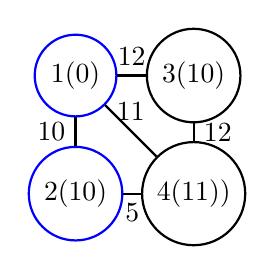
\begin{tikzpicture}[node distance={15mm}, thick, main/.style = {draw, circle}]
        \node[blue state] (1) {1(0)};
        \node[blue state] (2) [below of = 1] {2(10)};
        \node[main] (3) [right of = 1] {3(10)};
        \node[main] (4) [below of = 3]{4(11))};

        \draw[-] (1) -- (2) node [midway,left] {10};
        \draw[-] (2) -- (4) node [midway, below] {5};
        \draw[-] (3) -- (4) node [midway, right] {12};
        \draw[-] (1) -- (4) node [midway, right, above] {11};
        \draw[-] (1) -- (3) node [midway, above] {12};

    \end{tikzpicture}
\end{center}

\subparagraph*{Actualizam distantele vecinilor lui 2 si il luam pe minimul nevizitat (3)}

\begin{center}
    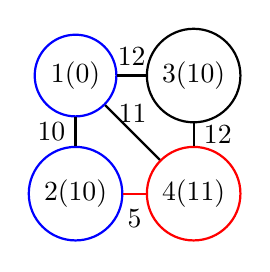
\begin{tikzpicture}[node distance={15mm}, thick, main/.style = {draw, circle}]
        \node[blue state] (1) {1(0)};
        \node[blue state] (2) [below of = 1] {2(10)};
        \node[main] (3) [right of = 1] {3(10)};
        \node[red state] (4) [below of = 3]{4(11)};

        \draw[-] (1) -- (2) node [midway,left] {10};
        \draw[red state] (2) -- (4) node [midway, below] {5};
        \draw[-] (3) -- (4) node [midway, right] {12};
        \draw[-] (1) -- (4) node [midway, right, above] {11};
        \draw[-] (1) -- (3) node [midway, above] {12};

    \end{tikzpicture}
\end{center}

\subparagraph*{Actualizam distantele vecinilor lui 2 si il luam pe minimul nevizitat (4)}

\begin{center}
    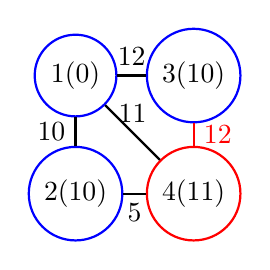
\begin{tikzpicture}[node distance={15mm}, thick, main/.style = {draw, circle}]
        \node[blue state] (1) {1(0)};
        \node[blue state] (2) [below of = 1] {2(10)};
        \node[blue state] (3) [right of = 1] {3(10)};
        \node[red state] (4) [below of = 3]{4(11)};

        \draw[-] (1) -- (2) node [midway,left] {10};
        \draw[-] (2) -- (4) node [midway, below] {5};
        \draw[red] (3) -- (4) node [midway, right] {12};
        \draw[-] (1) -- (4) node [midway, right, above] {11};
        \draw[-] (1) -- (3) node [midway, above] {12};

    \end{tikzpicture}
\end{center}

\subparagraph*{Luam minimul nevizitat si vedem ca nu mai are vecini}

\begin{center}
    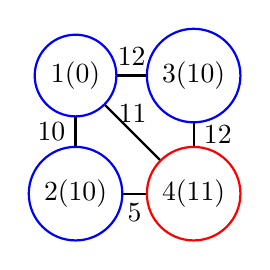
\begin{tikzpicture}[node distance={15mm}, thick, main/.style = {draw, circle}]
        \node[blue state] (1) {1(0)};
        \node[blue state] (2) [below of = 1] {2(10)};
        \node[blue state] (3) [right of = 1] {3(10)};
        \node[red state] (4) [below of = 3]{4(11)};

        \draw[-] (1) -- (2) node [midway,left] {10};
        \draw[-] (2) -- (4) node [midway, below] {5};
        \draw[-] (3) -- (4) node [midway, right] {12};
        \draw[-] (1) -- (4) node [midway, right, above] {11};
        \draw[-] (1) -- (3) node [midway, above] {12};

    \end{tikzpicture}
\end{center}

\paragraph*{Lema}
Pentru $\forall u\in V$, la orice pas al algoritmului lui Dijkstra avem:
\begin{itemize}
    \item dacă $d[u]<\infty$, există un drum de la s la u în G de cost d[u] și acesta se poate determina din vectorul tata: \\ tata[u]= predecesorul lui u pe un drum de la s la u de cost d[u]
    \item $d[u] \leq \delta(s,u)$
\end{itemize}
\subparagraph*{Consecinta} Dacă la un pas al algoritmului avem pentru un vârf u relația $d[u] = \delta(s, u)$, atunci d[u] nu se mai modifică până la final.

\paragraph*{Teorema} Fie G=(V, E, w) un graf orientat ponderat cu $w : E \to \mathbb{R}_+$ și $s \in V$ fixat.\\
La finalul algoritmul lui Dijkstra avem:
$d[u] = \delta(s, u)$ pentru orice $u \in V$ și tata memorează un arbore al distanțelor față de s.

\subsection*{Bellman-Ford}
Se poate folosi si pentru drumuri negative
\paragraph*{Complexitate} $O(V*E)$
\begin{center}
    \includegraphics[scale=0.3]{6_bellmanford.png}
\end{center}

\paragraph*{Optimizare} Se pot relaxa doar arcele din varfurile ale caror etichete s-au modificat anterior

\paragraph*{Exemplu}
\begin{center}
    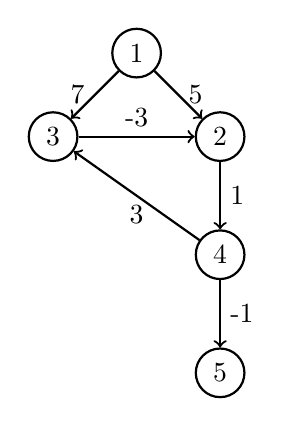
\begin{tikzpicture}[node distance={15mm}, thick, main/.style = {draw, circle}]
        \node[main] (1) {1};
        \node[main] (2) [below right of = 1] {2};
        \node[main] (3) [below left of = 1] {3};
        \node[main] (4) [below of = 2]{4};
        \node[main] (5) [below of = 4]{5};

        \draw[->] (1) -- (2) node [midway,right] {5};
        \draw[->] (1) -- (3) node [midway, left] {7};
        \draw[->] (2) -- (4) node [midway, right] {1};
        \draw[->] (4) -- (5) node [midway, right] {-1};
        \draw[->] (3) -- (2) node [midway, above] {-3};
        \draw[->] (4) -- (3) node [midway, below] {3};

    \end{tikzpicture}
\end{center}

\subparagraph*{Etapa 1}

\subparagraph*{Relaxam}
\begin{itemize}
    \item 1 2
    \item 1 3
\end{itemize}

\begin{center}
    \begin{tabularx}{0.8\textwidth} {
            | >{\centering\arraybackslash}X
            | >{\centering\arraybackslash}X
            | >{\centering\arraybackslash}X
            | >{\centering\arraybackslash}X
            | >{\centering\arraybackslash}X
            | >{\centering\arraybackslash}X
            |}
        \hline
          & 1 & 2                  & 3                  & 4        & 5        \\
        \hline
        d & 0 & \textcolor{red}{5} & \textcolor{red}{7} & $\infty$ & $\infty$ \\
        \hline
    \end{tabularx}
\end{center}

\subparagraph*{Relaxam}
\begin{itemize}
    \item 1 2
    \item 1 3
    \item 2 4
\end{itemize}

\begin{center}
    \begin{tabularx}{0.8\textwidth} {
            | >{\centering\arraybackslash}X
            | >{\centering\arraybackslash}X
            | >{\centering\arraybackslash}X
            | >{\centering\arraybackslash}X
            | >{\centering\arraybackslash}X
            | >{\centering\arraybackslash}X
            |}
        \hline
          & 1 & 2 & 3 & 4                  & 5        \\
        \hline
        d & 0 & 5 & 7 & \textcolor{red}{6} & $\infty$ \\
        \hline
    \end{tabularx}
\end{center}

\subparagraph*{Relaxam}
\begin{itemize}
    \item 1 2
    \item 1 3
    \item 2 4
    \item 4 3
    \item 4 5
\end{itemize}

\begin{center}
    \begin{tabularx}{0.8\textwidth} {
            | >{\centering\arraybackslash}X
            | >{\centering\arraybackslash}X
            | >{\centering\arraybackslash}X
            | >{\centering\arraybackslash}X
            | >{\centering\arraybackslash}X
            | >{\centering\arraybackslash}X
            |}
        \hline
          & 1 & 2 & 3 & 4 & 5                  \\
        \hline
        d & 0 & 5 & 7 & 6 & \textcolor{red}{5} \\
        \hline
    \end{tabularx}
\end{center}

\subparagraph*{Relaxam}
\begin{itemize}
    \item 1 2
    \item 1 3
    \item 2 4
    \item 4 3
    \item 4 5
    \item 3 2
\end{itemize}

\begin{center}
    \begin{tabularx}{0.8\textwidth} {
            | >{\centering\arraybackslash}X
            | >{\centering\arraybackslash}X
            | >{\centering\arraybackslash}X
            | >{\centering\arraybackslash}X
            | >{\centering\arraybackslash}X
            | >{\centering\arraybackslash}X
            |}
        \hline
          & 1 & 2                  & 3 & 4 & 5 \\
        \hline
        d & 0 & \textcolor{red}{4} & 7 & 6 & 5 \\
        \hline
    \end{tabularx}
\end{center}

\subparagraph*{Etapa 2}
\subparagraph*{Relaxam}
\begin{itemize}
    \item 2 4
\end{itemize}

\begin{center}
    \begin{tabularx}{0.8\textwidth} {
            | >{\centering\arraybackslash}X
            | >{\centering\arraybackslash}X
            | >{\centering\arraybackslash}X
            | >{\centering\arraybackslash}X
            | >{\centering\arraybackslash}X
            | >{\centering\arraybackslash}X
            |}
        \hline
          & 1 & 2 & 3 & 4 & 5                  \\
        \hline
        d & 0 & 5 & 7 & 6 & \textcolor{red}{5} \\
        \hline
    \end{tabularx}
\end{center}

\subparagraph*{Relaxam}
\begin{itemize}
    \item 2 4
    \item 4 3
\end{itemize}

\begin{center}
    \begin{tabularx}{0.8\textwidth} {
            | >{\centering\arraybackslash}X
            | >{\centering\arraybackslash}X
            | >{\centering\arraybackslash}X
            | >{\centering\arraybackslash}X
            | >{\centering\arraybackslash}X
            | >{\centering\arraybackslash}X
            |}
        \hline
          & 1 & 2 & 3 & 4 & 5 \\
        \hline
        d & 0 & 5 & 7 & 6 & 5 \\
        \hline
    \end{tabularx}
\end{center}

\subparagraph*{Relaxam}
\begin{itemize}
    \item 2 4
    \item 4 3
    \item 4 5
\end{itemize}

\begin{center}
    \begin{tabularx}{0.8\textwidth} {
            | >{\centering\arraybackslash}X
            | >{\centering\arraybackslash}X
            | >{\centering\arraybackslash}X
            | >{\centering\arraybackslash}X
            | >{\centering\arraybackslash}X
            | >{\centering\arraybackslash}X
            |}
        \hline
          & 1 & 2 & 3 & 4 & 5                  \\
        \hline
        d & 0 & 5 & 7 & 6 & \textcolor{red}{4} \\
        \hline
    \end{tabularx}
\end{center}

\subparagraph*{Relaxam}
\begin{itemize}
    \item 2 4
    \item 4 3
    \item 4 5
    \item 3 2
\end{itemize}

\begin{center}
    \begin{tabularx}{0.8\textwidth} {
            | >{\centering\arraybackslash}X
            | >{\centering\arraybackslash}X
            | >{\centering\arraybackslash}X
            | >{\centering\arraybackslash}X
            | >{\centering\arraybackslash}X
            | >{\centering\arraybackslash}X
            |}
        \hline
          & 1 & 2 & 3 & 4 & 5 \\
        \hline
        d & 0 & 5 & 7 & 6 & 4 \\
        \hline
    \end{tabularx}
\end{center}

\subparagraph*{Etapa 3}
\subparagraph*{Relaxam}
\begin{itemize}
    \item 2 4
    \item 4 3
    \item 4 5
    \item 3 2
\end{itemize}

\begin{center}
    \begin{tabularx}{0.8\textwidth} {
            | >{\centering\arraybackslash}X
            | >{\centering\arraybackslash}X
            | >{\centering\arraybackslash}X
            | >{\centering\arraybackslash}X
            | >{\centering\arraybackslash}X
            | >{\centering\arraybackslash}X
            |}
        \hline
          & 1 & 2 & 3 & 4 & 5 \\
        \hline
        d & 0 & 5 & 7 & 6 & 4 \\
        \hline
    \end{tabularx}
\end{center}

\textbf{Nu se mai actualizeaza nimic. Ne oprim}

\paragraph*{Lema}
Pentru $\forall u\in V$, la orice pas al algoritmului lui Bellman-Ford avem:
\begin{itemize}
    \item dacă $d[u]<\infty$, există un drum de la s la u în G de cost d[u] și acesta se poate determina din vectorul tata: \\ tata[u]= predecesorul lui u pe un drum de la s la u de cost d[u]
    \item $d[u] \leq \delta(s,u)$
\end{itemize}

\paragraph*{Detectarea de circuite negative}
\begin{center}
    \includegraphics[scale=0.3]{7_bellmanford_circneg.png}
\end{center}

\subparagraph*{Algoritm}Afișarea ciclului negative detectat - folosind tata:
\begin{itemize}
    \item Fie v un vârf al cărei etichetă s-a actualizat la pasul k
    \item  Facem n pași înapoi din v folosind vectorul tata (către s) ; fie x vârful în care am ajuns
    \item Afișăm ciclul care conține pe x folosind tata (din x până ajungem iar în x)
\end{itemize}

\subsection*{Drumuri minime de sursa unica in grafuri aciclice}
\begin{center}
    \includegraphics[scale=0.3]{8_drumminim_sursaunica.png}
\end{center}

\paragraph*{Complexitate} $O(V+E)$
\begin{itemize}
    \item Initializare: $O(n)$
    \item Sortare topologica: $O(m+n)$
    \item m * relaxare uv: $O(m)$
\end{itemize}

\section{Drumuri minime intre toate perechile de varfuri}
\subsection*{Floyd-Warshall}
\paragraph*{Complexitate} $O(n^3)$

\begin{lstlisting}
for(i=1;i<=n;i++)
    for(j=1;j<=n;j++){
        d[i][j]=w[i][j]; // adaugam distanta ca fiind greutatea muchiei
        // daca e INF, nu e parinte, altfel il adaugam
        if(w[i][j]== INF)
            p[i][j]=0;
        else
            p[i][j]=i;
    }

    for(k=1;k<=n;k++)
        for(i=1;i<=n;i++)
            for(j=1;j<=n;j++)
                if(d[i][j]>d[i][k]+d[k][j]){ 
                    // Daca ce avem e mai mare decat suma distantelor, actualizam
                    d[i][j]=d[i][k]+d[k][j];
                    p[i][j]=p[k][j];
                }
   \end{lstlisting}

\begin{center}
    \includegraphics[scale=0.3]{9_floydwarshall.png}
\end{center}

\paragraph*{Inchiderea tranzitiva}
\begin{center}
    \begin{lstlisting}
for(k=1;k<=n;k++)
    for(i=1;i<=n;i++)
        for(j=1;j<=n;j++)
            d[i][j] = d[i][j] || (d[i][k] && d[k][j]);
        \end{lstlisting}
\end{center}

\section{Flow}
\subsection*{Ford Fulkerson}
\paragraph*{Exemplu}




\end{document}